\chapter{Background \& Foundations}\label{chap:k2}

\section{Partial Differential Equations}
Since the paper resolves around solving PDEs with neural networks, 
at first it is important to understand what exactly a PDE is. 
A PDE is an equation with multiple variables and involves its partial derivatives. 
The most common example is the one dimensional wave equation explaining the motion of a wave over time: 
\[\frac{\partial^2u}{\partial t^2} = c^2 \frac{\partial^2u}{\partial x^2}\]
with c being a constant, or in our case a variable PDE parameter~\cite{olver2014introduction}. \\
\[\frac{\partial^2u}{\partial t^2}\] 
is the notation for the second derivative of u after t, while 
\[\frac{\partial^2u}{\partial x^2}\] 
is the notation for the second derivative of u after x. 
Usually, PDEs have multiple solutions. 
In order to restrict the results, and in the best case to arrive at a unique one, 
PDEs require one initial conditions, which define an initial value. 
They also require boundary conditions, 
which define how the PDE should behave at the limits of the domain~\cite{borthwick2017introduction}.
\section{Active learning}
Active learning is a subfield of machine learning 
where the model is able to choose the data it wants to learn from. 
In typical machine learning, the unlabeled instances are chosen randomly. 
This method works, but with active learning the cost of labeling decreases, 
resulting in a more efficient model~\cite{ramirez2017active}.
 Specifically, the model can query an unlabeled data from an oracle,
  which then labels it~\cite{settles2009active}. 
There are three main approaches, all 
visualised in a very simplified way in Fig.~\ref{fig:AL-overview}. 
\begin{figure}
    \centering
    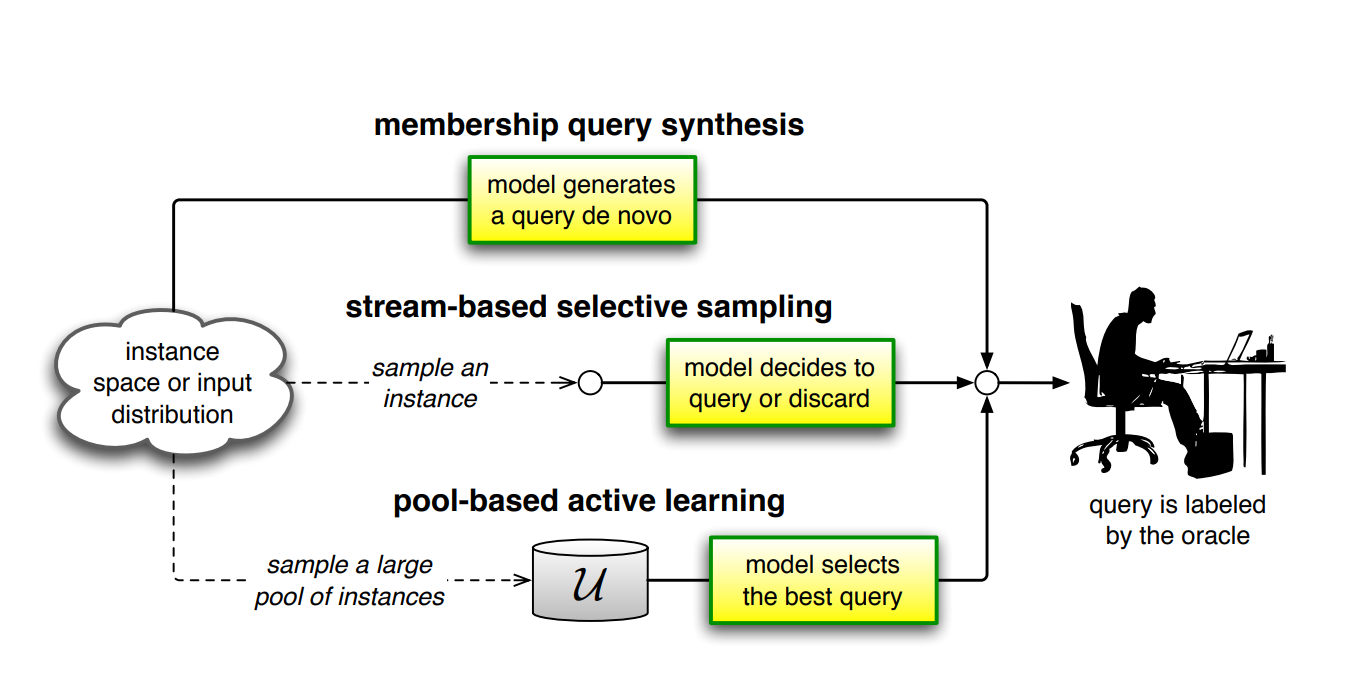
\includegraphics[width=1\linewidth]{../graphics/active_learning.png}
    \caption{The three main methods of active learning by Settels~\cite{settles2009active}}.
    \label{fig:AL-overview}
\end{figure}
\subsection{Pool-based active learning}
The pool-based approach is about sampling a large pool 
of unlabeled instances from the original instance 
space/input distribution. Samples from this pool then 
get queried to an oracle which will generate a label, 
visualized in Fig. \ref{fig:AL-pool}.
In mathematical terms, we will reuse the 
definition from Ren et al.~\cite{ren2021survey}. 
Let $U^n = \{\X, \Y\}$ be the unlabeled dataset with n samples,
with $\X$ being the sample size and $\Y$ being the label size.
P(x,y) is a potential distribution, with $x \in \X$, $y \in \Y$. 
It represents the joint probability distribution of the sample 
$x$ and the label $y$. $L^m=\{X,Y\}$ is the training set with m labeled instances. 
Now the goal is to create a query strategy Q, 
which queries samples from $U^n$ to be labeled 
by the oracle: $U^n \xrightarrow{\text{Q}} L^m$. 
The most common query strategy is 
to select the instances the model has the least certainty in.
This approach is called "Uncertainty-based",
and is simple to implement and most importantly, 
it frequently improves over random sampling~\cite{zhan2021comparative}. 
In context of deep active learning, the combination of deep learning 
and active learning, uncertainty-based methods reaches it limits 
since single points do not have a statistically significant 
impact and a full iteration of the deep-learning network is 
required to train each data point~\cite{sener2017active}. 

\subsection{Batch active learning}
When training a deep-learning network with a pool-based approach, 
it is inefficient to query single points. 
In batch active learning, instead of a single point, 
a whole batch of size $K$ with $K\in\mathcal{N}$  
is selected from the given pool~\cite{ren2021survey}. 
Each time new points are selected, an initial batch of 
unlabeled data samples 
$\mathcal{B} = \{x_1,x_2,...,x_b\}\subseteq U$ 
based on a function $a$ is selected. 
\subsection{Stochastic batch active learning}
As in normal uncertainty-based pool-based active learning, 
an usual acquisition function to select the batch is 
through the uncertainty of the model with the difference 
of selecting the $K$ highest points instead of a singular point: 
\[
a_s^{\text{batch}}(\mathcal{I}^{\text{train}};K) := arg\,max_{I\subseteq\mathcal{I}^{\text{pool}},\lvert I\rvert = K}\sum_{i\in I}s(i;\mathcal{I}^{\text{train}})
\]    
with $a$ being the acquisition function, 
$\mathcal{I}^{\text{train}}$ being the indices of the samples 
in the training data set and $\mathcal{I}^{\text{pool}}$ being the indices 
of the samples in the pool data set~\cite{kirsch2021stochastic}.\\
Since only selecting the Top-$K$ instances can lack diversity, 
Kirsch et al.~\cite{kirsch2021stochastic} introduce stochastic batch 
active learning (SBAL). SBAL samples without replacement the input 
$\psi$ from the pool $S_{\text{pool}}$ with the probability distribution 
$p_{\text{power}(\psi)}\propto\alpha(\psi)^m$  with $m$ being a 
hyperparameter, that is controlling the sharpness of the distribution.

\begin{figure}
    \centering
    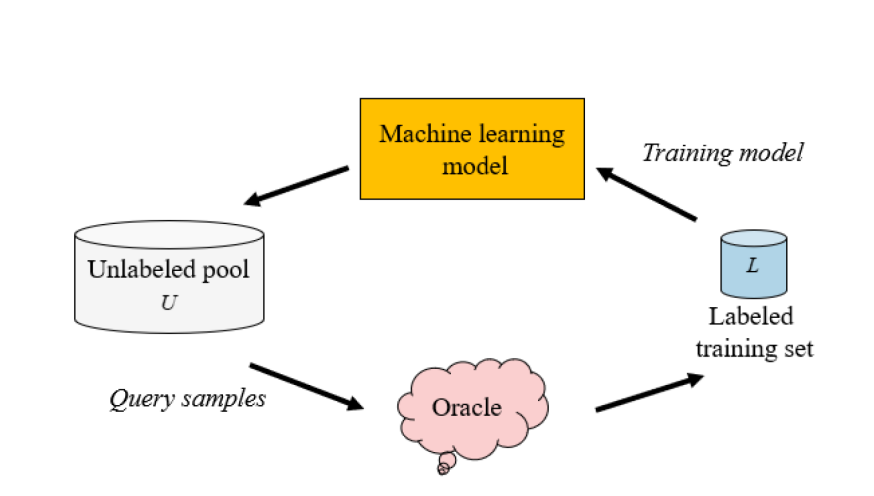
\includegraphics[width=1\linewidth]{../graphics/pool-based.png}
    \caption{The pool-based cycle done by Ren et al.~\cite{ren2021survey}}
    \label{fig:AL-pool}
\end{figure}


\subsection{Query synthesis active learning}
Query synthesis active learning (QSAL), 
or membership query synthesis active learning 
is another approach for active learning. 
Instead of sampling a large pool of instances 
like in pool-based active learning, 
the algorithm can query directly from the input space, 
or can create new queries. Because we do not need to 
evaluate the pool over and over again, making the 
algorithm more efficient. The algorithm is also more versatile, 
as we don't have to take samples from the pool to which we are bound~\cite{wang2015active}.
\section{Markov chain Monte Carlo}
Markov chain Monte Carlo (MCMC) is a class of algorithms 
for posterior sampling~\cite{wang2020brief}. 
Posterior sampling means sampling from a posterior distribution \[
\pi(\theta|y)=\frac{\pi(y|\theta)\pi(\theta)}{\pi(y)}
\]
with y being the data to be modeled, $\pi(y|\theta)$ 
being the distribution of $y$ and $\pi(\theta)$ 
being the density of the prior $\theta$.
MCMC samples from this distribution by creating a Makrov chain. 
The Makrov chain is discrete-time and constructed in a way so each sample 
has the same distribution. To achieve a stationary distribution, 
it starts with a selected distribution and is run until convergence. 
The first n states without stationary distributions are called 
burn-in and all values are discarded. Because the samples are 
related to each other MCMC is a dependent sampling method.
One general way of constructing the Markov chain is the 
Metropolis-Hastings algorithm, which performs a controlled 
random walk over the parameter space to ensure the Markov
chain has the posterior distribution as its stationary distribution~\cite{wang2020brief}. 

MCMC is not the only possible algorithm for posterior sampling. 
Another way for posterior sampling is Variational Inference. 
For example Local Refinement, a method created by 
Havasi et al.~\cite{havasi2021sampling}. 
To get close to the posterior, 
it starts with a mean-field approximation and then refines it 
locally with inexpensive operatioxns. From that refined region, 
it is possible to generate samples.
\subsection{Metropolis-Hastings algorithm}
The Metropolis-Hastings algorithm is one possible implementation of constructing the Makrov chain in MCMC and 
is developed by Hastings~\cite{hastings1970}.
Let $\pi(x)$ be the density we want to take samples from, called the target density.
Then, the algorithm requires a distribution proportional to the target denisity, $\pi(x)\propto\tilde{\pi}(x)$.
To determine the next state in the Makrov chain, it also requires a proposal kernal $q$.

The transition from the Makrov state $X_t$ to $X_{t+1}$ is then defined as follows.
Sample a new State  $X_{t+1}$ from $q(y | X_t)$. 
Accept or reject the State with the acceptance probability
\[ 
    \alpha(X_t, X_{t+1}) = 
    \begin{cases}
        \min \left\{ \frac{\tilde{\pi}(X_{t+1}) q(X_t|X_{t+1} )}{\tilde{\pi}(X_t) q(X_{t+1}|X_t)}, 1 \right\} & \text{if } \tilde{\pi}(X_t)q(X_{t+1}|X_t)>0 \\
        1 & \text{otherwise}
    \end{cases}     
\]
If accepted, then set $X_{t+1}=X_{t+1}$, otherwise $X_{t+1}  = X_t$ and restart the process.

Metropolis-Hastings is a further developlment of the Metropolis algorithm, which was introduced by Metropolis et al.~\cite{metropolis1953} and required $q$ to be symmetrical.

In Random Walk Metropolis, the proposals are drawn with i.i.d and fixed symmetric densities $Z_i$,
for example $Z_i\sim N(0,\sigma^2 I_d)$.
Each new proposal therefore has the form $X_{i+1} = X_i + Z_{i+1}$~\cite{rosenthal2011optimal}.
\todo{Umschreiben und Quelle wechseln}
\subsection{Hamiltonian Dynamics}
\todo{Ausformulieren}
-originated from physics
-important formulas
\subsection{Hamiltonian Monte Carlo}
Hamiltonian Monte Carlo is an adaptation of Metropolis-Hastings, which uses 
Hamiltonian dynamics to sample from a unknown distribution, in bayesian conext the posterior distribution.
It was originally published under the name of Hybrid Monte Carlo by Duane et al.~\cite{DUANE1987216}, but 
it became known under the name of Hamiltonian Monte Carlo, due to the more specific formulation.
Since Hamiltonian dynamics normally occurs in the physical context, the terms are also adopted in the machine learning context.

As we saw in the previous section , Hamiltonian dynamics require two $d$-dimensional vectors, one describing the position $q_i$, with $i=1,...,d$ entries. 
The vector here is the one we want to sample from, and consists in difference to normal Hamiltonian dynamics out of the network parameters. 
\begin{align*}
    \frac{dq_i}{d_t}&=\frac{\partial H}{\partial p_i} \\
    \frac{dp_i}{d_t}&=-\frac{\partial H}{\partial q_i}
\end{align*}

for $i=1,...,d$~\cite{MR2858447}. 


  

\begin{itemize}
    \item p two dimensional vektor momentum -> $m\cdot v$
    \item q two dimensional vektor position 
    \item $U(q)$ potential energy $U(q)\propto$ height of surface and kinetic energy
    \item kinetic energy $K(p)=\frac{\abs{p}^2}{2m}$
    \item constant velocity $v=\frac{p}{m}$
\end{itemize}   
\subsection{Metropolis adjusted Langevin algorithm}
 
similar to RMW, but proposal increment distribution $Z_i$ is defined as 
\[
Z_i \sim N((X_N?)\frac{\sigma^2}{2}\nabla\log\pi(X_n),\sigma^2I_d)
\]
optimal acceptance rate $A(l_{opt})=0.574$

\listoftodos[Todos here]